\section{Řídící jednotka}\label{sec:ridici-jednotka}
Řídící jednotka je vlastní sestavené zařízení, které zprostředkovává pomocí USB připojení data o teplotě a vlhkosti v kurníku.
Další úlohou je ovládání dvířek a světla.
Srdem řídící jednotky je Arduino Nano.
Tento programovatelný mikrokontroler slouží jako logický prvek mezi nízkoúrovňovími prvky(relé, senzory, táhlový motor) a počítačem, na němž běží služby ovládají nebo využívající data z těchto prvků.

\subsection*{Popis zapojení}
Zapojení řídící jednotky je zdokumentováno na obrázku~\ref{fig:ridici_jednotka} a blokové schéma zapojení je na obrázku~\ref{fig:schema_ridici_jednotky}.
Vezkratce, jak již bylo zmíněno, je řídící jednotka složena z několika částí.
\begin{itemize}
    \item mikrokontroler Arduino Nano v3.0
    \item senzor DHT11 pro teplotu a vlhkost
    \item relé s napětím cívky 5 V a spínacím proudem 10 A stejnosměrných
\end{itemize}
Pro snadnou práci s jednotlivými součástmi během vývoje, byly zvoleny moduly, které disponují svorkovnicemi a není tedy nutné k nim nic pájet.
Připojení Ardruina je realizováno pomocí terminal schieldu, který pro každý pin desky disponuje jednou svorkou pro připojení kabelu.
Obdobně byl pro práci s relátky vybrán modul osazený již 4 relátky a samozřejmě svorkovnicí pro snadné zapojení.
Nejkomplikovanější byl modul snímače ke kterému bylo třeba vytvořit konektor protože disponoval pouze výstupními piny.
Po pečlivém vybrání a sehnání všech součástí byla zvolena dřevotřísková deska jako platforma na níž se naistalují všechny moduly pomocí krátkých vrutů do dřeva.
Jednotlivé moduly byli následně propojeny kablíky o průřezu 0,15 mm² dle technické dokumentace dodávané ke každému modulu.
Hardwarová stránka byla tímto hotová.
\newline
Arduino a ostatní periferie se napájí skrze USB port Arduina, takže nebylo třeba řešit, žádné přídavné napájení.
Přídavné napájení by bylo třeba řešit například, kdybychom používali 10 relejových modulů současně, protože limit pro napájení skrze USB 2.0 je pouze 500 mA a jedna cívka spotřebuje až 70 mA.\newline
Následovala tedy poslední věc a to nahrád kód programu do samotné vývojové desky Arduno Nano.
K tomu to účelu jsem využil open-source vývojářského nástroje Arduino IDE, který celý složitý proces nahrávání vyřeší.

\begin{figure}[htbp]
    \centering
    % První řádek
    \begin{minipage}[b]{0.45\textwidth}
        \centering
        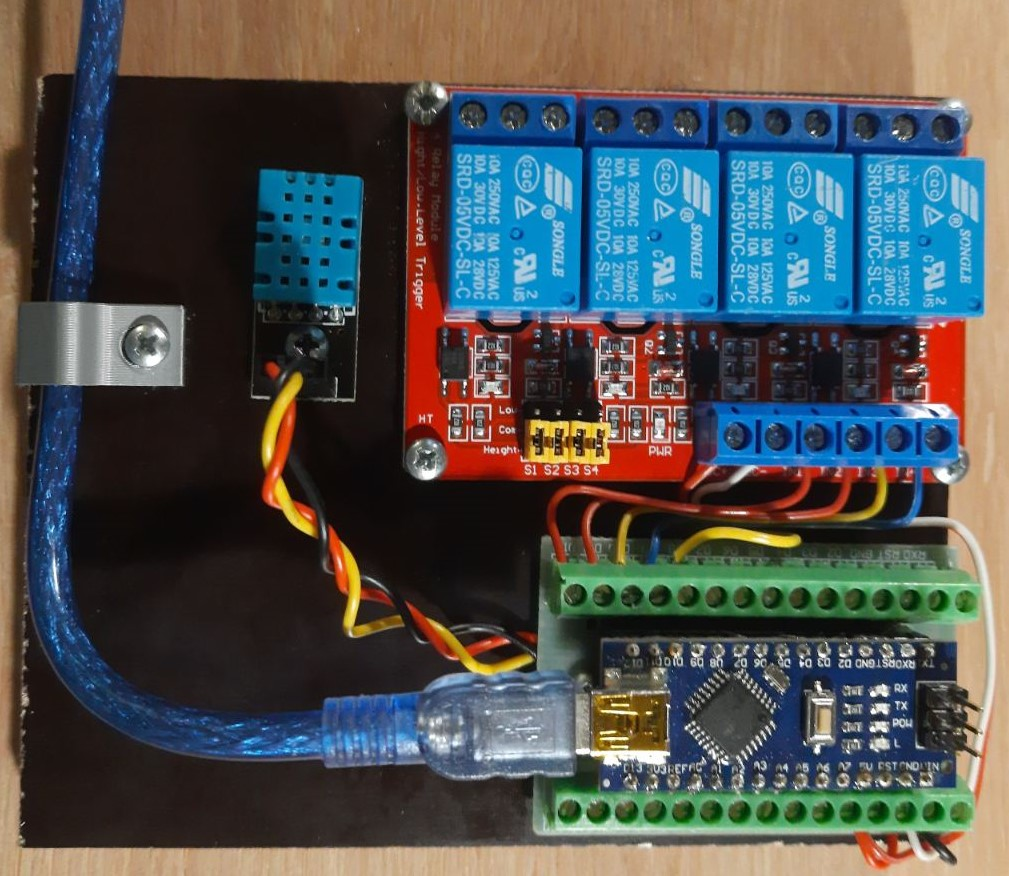
\includegraphics[width=\textwidth]{img/ridici_jednotka}
        \caption{Výsledek detekce slepic 1}
        \label{fig:ridici_jednotka}
    \end{minipage}
    \hfill
    \begin{minipage}[b]{0.45\textwidth}
        \centering
        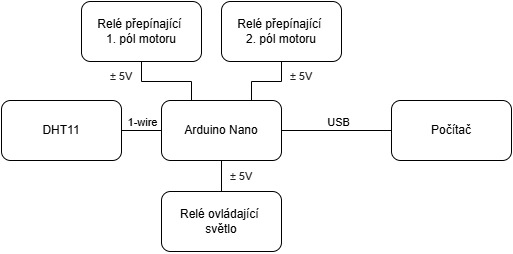
\includegraphics[width=\textwidth]{img/schema_ridici_jednotky}
        \caption{Výsledek detekce slepic 2}
        \label{fig:schema_ridici_jednotky}
    \end{minipage}
\end{figure}

\subsection*{Popis algoritmu}
V části programu Setup se jako první po startu programu nastavý příslušné módy na vstupní a výstupní piny.
Následně se provede inicializace seriálového připojení s rychlostí 9600 baudů.
Poté se inicializuje připojení s čidlem DHT11 pomocí knihovny DHT.h a na závěr jsou nastaveny výstupy dle aktuálních stavů řídících neboli stavových proměnných pro dvířka a světlo.
Dále program pokračuje do části Loop, což je metoda, která se volá pořád dokola jako nekonečný cyklus.
Tato metoda řeší pravidelnou aktualizaci dat ze senzoru dále čtení příkazů ze seriálového připojení a posílání odpovědí na ně.
Aktualizace senzorových dat se provádí jednou do vteřiny za pomocí mětod readTemperature a readHumidity, které jsou součástí knihovny DHT.h.
Zpracování příkazů probíhá zavoláním metody processCommand, která pokud je v zásobníku přijatých dat něco ke čtení, přečte první znak a ten následně zpracuje jako příkaz dle seznamu níže.

\subsection*{Seznam příkazů ovládacího protokolu}
\begin{itemize}
    \item o = otevřít dvířka
    \item c = zavřít dvířka
    \item l = rozsvítit světlo
    \item d = zhasnout světlo
    \item j = vrátí json s daty o teplotě a vlhkosti
    \item s = vrátí json s daty o stavech jednotlivých ovládaných prvku (dvěře, světlo)
\end{itemize}

%## funkcionalita
%- umoznuje ovladat osvetleni kurniku
%- resi otevírání a zavírání dvířek v kurníku
%- ziskava informace ze senzoru o teplote a vlhkosti v kurniku
%- komunikuje se zbytkem systému pomocí rest api
%- s arduinem komunikuje pomocí serialového portu a pomocí zasílání příkazů v podobě jednoho písmene
%- příkazy: o = otevřít dvířka, c = zavřít dvířka, l = rozsvítit světlo, d = zhasnout světlo, j = vrátí json s daty o teplotě a vlhkosti, s = vrátí json s daty o stavech jednotlivých ovládaných prvku (dvěře, světlo)
%
%## technologie
%- c++ / wire (jazyk pro programování v arduino ide)
%- knihovny pro arduino
%- defaultní **Arduino.h**
%- **DHT**: pro ovládání teplotních+vlhkostních sezorů DHT11 a DHT22
%- táhlový motor 12v nevím kolik neutonů
%- zpřevodovaný motorek k navijáku
%- relé 5v 10A
%
%
%## hardware
%- arduino Nano v3.0
%- teplotni a vlhkosti senzor DHT11
%- relatko ovladajici svetlo a relátka udávající chod a směr motoru
%- napájeno připojením ke raspberry pi přes usb napětím 5V
%